 
% ════════════════════════════════════════════════════════════════════════════
\chapter{Réalisation de l'interface SmartPlayAI}
% ════════════════════════════════════════════════════════════════════════════
 
\section{Introduction}
 
Ce chapitre est consacré à la réalisation concrète de l'interface utilisateur \textbf{SmartPlayAI},
le système d'analyse tactique et biométrique automatisée de matchs de padel développé dans le
cadre de ce projet de fin d'études. Après avoir présenté dans les chapitres précédents le
contexte applicatif, l'état de l'art des techniques de vision par ordinateur et l'architecture
générale du système, nous décrivons ici la couche applicative qui constitue le point d'entrée
de l'utilisateur vers ces modules d'intelligence artificielle : charger une vidéo de match,
configurer les paramètres d'analyse, déclencher le traitement neuronal, puis visualiser et
exploiter les résultats produits sous forme de rapport tactique interactif.
 
L'interface SmartPlayAI a été conçue selon une philosophie centrée sur l'expérience utilisateur :
rendre accessibles des algorithmes complexes — détection par réseau de neurones YOLO, calcul
d'homographie, télémétrie de mouvement, classification de frappes — à travers des commandes
claires, visuellement lisibles et organisées en un workflow guidé. Ce chapitre présente les
objectifs fonctionnels retenus, les choix de conception (diagrammes de cas d'utilisation et de
séquences), les technologies mobilisées, les différentes vues de l'interface et enfin le
workflow complet d'un utilisateur type.
 
% ════════════════════════════════════════════════════════════════════════════
\section{Objectifs et spécifications fonctionnelles}
% ════════════════════════════════════════════════════════════════════════════
 
L'interface SmartPlayAI répond à un ensemble de besoins fonctionnels identifiés lors de la phase
d'analyse des exigences, en concertation avec les utilisateurs cibles (entraîneurs de padel,
analystes sportifs). Ces besoins ont été organisés en deux catégories : fonctionnalités
primaires et fonctionnalités secondaires.
 
\subsection*{Fonctionnalités primaires (Must-Have)}
 
\begin{table}[H]
  \centering
  \renewcommand{\arraystretch}{1.3}
  \begin{tabularx}{\textwidth}{C{1.2cm} X C{2.5cm}}
    \rowcolor{tablehead}
    \textcolor{white}{\textbf{ID}} &
    \textcolor{white}{\textbf{Fonctionnalité}} &
    \textcolor{white}{\textbf{Priorité}} \\
    \rowcolor{rowalt}
    F01 & Chargement et synchronisation d'une vidéo de match (.mp4) & Haute \\
    F02 & Capture manuelle d'une frame annotée pour calibration du terrain & Haute \\
    \rowcolor{rowalt}
    F03 & Saisie ou import de keypoints de référence du terrain (JSON) & Haute \\
    F04 & Déclenchement du pipeline d'analyse neuronale complet & Haute \\
    \rowcolor{rowalt}
    F05 & Affichage du rapport tactique (KPIs, statistiques, graphiques) & Haute \\
    F06 & Suivi en temps réel de l'état du traitement (journal de mission) & Haute \\
  \end{tabularx}
  \caption{Fonctionnalités primaires de l'interface SmartPlayAI}
  \label{tab:fonctionnalites_primaires}
\end{table}
 
\subsection*{Fonctionnalités secondaires (Nice-to-Have)}
 
\begin{table}[H]
  \centering
  \renewcommand{\arraystretch}{1.3}
  \begin{tabularx}{\textwidth}{C{1.2cm} X C{2.5cm}}
    \rowcolor{tablehead}
    \textcolor{white}{\textbf{ID}} &
    \textcolor{white}{\textbf{Fonctionnalité}} &
    \textcolor{white}{\textbf{Priorité}} \\
    \rowcolor{rowalt}
    F07 & Comparaison côte à côte de deux joueurs (Player Comparison) & Moyenne \\
    F08 & Heatmap 2D de présence sur le terrain (3D Arena Heatmap) & Moyenne \\
    \rowcolor{rowalt}
    F09 & Historique des analyses récentes (Recent Operations) & Basse \\
    F10 & Export du rapport en format structuré (JSON / MP4 annoté) & Basse \\
  \end{tabularx}
  \caption{Fonctionnalités secondaires de l'interface SmartPlayAI}
  \label{tab:fonctionnalites_secondaires}
\end{table}
 
L'interface doit également satisfaire les contraintes non-fonctionnelles suivantes :
 
\begin{itemize}[leftmargin=1.5em]
  \item \textbf{Réactivité} : retour visuel immédiat lors de toute interaction utilisateur
        (chargement, analyse, navigation)
  \item \textbf{Lisibilité} : affichage des métriques dans un format tabulaire et graphique
        clair, avec hiérarchie visuelle
  \item \textbf{Modularité} : les vues sont indépendantes et navigables via une barre de
        navigation supérieure
  \item \textbf{Compatibilité} : accessible via navigateur web standard (Chrome, Firefox)
        sans installation cliente
  \item \textbf{Robustesse} : gestion explicite des erreurs de pipeline avec retour
        d'information dans le journal de mission
\end{itemize}
 
% ════════════════════════════════════════════════════════════════════════════
\section{Conception}
% ════════════════════════════════════════════════════════════════════════════
 
\subsection{Diagramme de cas d'utilisation}
 
Le diagramme de cas d'utilisation ci-dessous représente les interactions entre les deux acteurs
principaux du système et les grandes fonctionnalités de l'interface SmartPlayAI.
 
\medskip
\noindent\textbf{Acteurs identifiés :}
\begin{itemize}[leftmargin=1.5em]
  \item \textbf{Utilisateur} : acteur principal (entraîneur / analyste) qui pilote l'ensemble
        du workflow — il charge la vidéo, configure les paramètres et consulte les résultats.
  \item \textbf{Système} : acteur secondaire représentant le backend de traitement, qui prend
        en charge la génération des analyses et l'affichage des résultats.
\end{itemize}
 
% ─────────────────────────────────────────────────────────────────────────────
% FIGURE 4.1 — Diagramme de cas d'utilisation
% Remplacez VOTRE_URL_IMAGE_4_1 par l'URL ou le chemin local de l'image
% ─────────────────────────────────────────────────────────────────────────────
\begin{figure}[H]
    \centering
      \maybeincludegraphics[width=0.9\textwidth]{images_chap3/Utilisateur.png}
    \caption{Diagramme de cas d'utilisation}
    \label{fig:casdutilisation}
\end{figure}
 
Le diagramme distingue deux groupes de cas d'utilisation selon l'acteur qui les initie :
 
\subsubsection*{Cas d'utilisation initiés par l'utilisateur}
 
\begin{itemize}[leftmargin=1.5em]
  \item \textbf{UC1 – Charger une vidéo} : L'utilisateur sélectionne et importe un fichier
        \texttt{.mp4} dans le panneau de configuration. Le backend valide le flux vidéo,
        transcode si nécessaire via \texttt{ffmpeg}, et confirme la synchronisation.
 
  \item \textbf{UC2 – Définir les keypoints ou charger un fichier JSON} : L'utilisateur saisit
        manuellement les coordonnées des 12 points de référence du terrain ou importe un fichier
        \texttt{.json} de calibration préalablement établi.
 
  \item \textbf{UC3 – Visualisation des résultats} : L'utilisateur consulte le rapport tactique
        complet — KPIs globaux, statistiques individuelles, télémétrie et classification des
        frappes.
 
  \item \textbf{UC4 – Consulter l'historique des analyses} : L'utilisateur accède aux analyses
        précédentes archivées via leurs identifiants hexadécimaux (bloc \textit{Recent
        Operations}) pour un suivi longitudinal.
\end{itemize}
 
\subsubsection*{Cas d'utilisation pris en charge par le système}
 
\begin{itemize}[leftmargin=1.5em]
  \item \textbf{UC5 – Visualisation de contenu visuel} : Le système génère et affiche la frame
        annotée extraite de la vidéo.
 
  \item \textbf{UC6 – Générer des analyses} : Le système exécute le pipeline complet
        (PlayersTracker, BallTracker, KeypointsTracker, DataAnalytics).
 
  \item \textbf{UC7 – Afficher les analyses} : Le système formate et restitue les résultats
        dans le tableau de bord tactique interactif.
\end{itemize}
 
% ────────────────────────────────────────────────────────────────────────────
\subsection{Diagramme de séquences}
% ────────────────────────────────────────────────────────────────────────────
 
Le diagramme de séquence suivant décrit le flux d'interactions lors d'un scénario nominal
complet, structuré en cinq phases distinctes. Il implique quatre participants :
l'\textbf{Utilisateur}, l'\textbf{Interface (React)}, le \textbf{Serveur (FastAPI)} et le
\textbf{Cloud (Desktop)} qui héberge les données d'analyse.
 
% ─────────────────────────────────────────────────────────────────────────────
% FIGURE 4.2 — Diagramme de séquence
% Remplacez VOTRE_URL_IMAGE_4_2 par l'URL ou le chemin local de l'image
% ─────────────────────────────────────────────────────────────────────────────
\begin{figure}[H]
    \centering
      \maybeincludegraphics[width=0.9\textwidth]{images_chap3/sequence.png}
    \caption{Diagramme de séquence : flux complet d'une analyse SmartPlayAI}
    \label{fig:sequence}
\end{figure}

Le scénario se déroule selon les cinq phases suivantes :
 
\subsubsection*{Phase 1 — Initialisation du serveur}
Avant toute interaction utilisateur, le serveur FastAPI effectue une opération préalable :
\begin{itemize}[leftmargin=1.5em]
  \item \textbf{Étape 1} : Le serveur charge automatiquement toutes les données d'analyse
        disponibles depuis le stockage Cloud (Desktop), initialisant ainsi le contexte de
        session.
\end{itemize}
 
\subsubsection*{Phase 2 — Préparation du contenu}
L'utilisateur importe la source vidéo à analyser :
\begin{itemize}[leftmargin=1.5em]
  \item \textbf{Étape 2} : L'utilisateur importe une vidéo depuis l'interface React.
  \item \textbf{Étape 3} : L'interface transfère le fichier vidéo au serveur FastAPI pour
        traitement.
  \item \textbf{Étape 4} : Le serveur confirme le chargement de la vidéo à l'interface
        (réponse synchrone).
\end{itemize}
 
\subsubsection*{Phase 3 — Lancement de l'analyse}
L'utilisateur déclenche le pipeline de traitement :
\begin{itemize}[leftmargin=1.5em]
  \item \textbf{Étape 5} : L'utilisateur clique sur le bouton \textbf{"Démarrer Traitement"}.
  \item \textbf{Étape 6} : L'interface initialise l'affichage de l'analyse (activation du
        journal de mission).
\end{itemize}
 
\subsubsection*{Phase 4 — Synchronisation et affichage des résultats (boucle)}
Cette phase s'exécute en boucle \textbf{pour chaque paire de frames pertinente} de la vidéo :
\begin{itemize}[leftmargin=1.5em]
  \item \textbf{Étape 7} : L'interface demande au serveur les métriques d'homographie pour la
        paire de frames courante.
  \item \textbf{Étape 8} : Le serveur récupère les correspondances de points depuis le Cloud
        (Desktop).
  \item \textbf{Étape 9} : Le Cloud fournit les données de points au serveur.
  \item \textbf{Étape 10} : Le serveur calcule et fournit les métriques d'homographie à
        l'interface.
  \item \textbf{Étape 11} : L'interface affiche les métriques calculées à l'utilisateur en
        temps réel.
\end{itemize}
 
\subsubsection*{Phase 5 — Fin de l'analyse}
\begin{itemize}[leftmargin=1.5em]
  \item \textbf{Étape 12} : L'interface termine le scénario d'analyse et notifie l'utilisateur
        que le rapport complet a été généré et est disponible dans le tableau de bord tactique.
\end{itemize}
 
% ════════════════════════════════════════════════════════════════════════════
\section{Choix technologiques}
% ════════════════════════════════════════════════════════════════════════════
 
\subsection{Environnement matériel}
 
Le développement et les tests de l'interface SmartPlayAI ont été réalisés sur la configuration
matérielle suivante :
 
\begin{table}[H]
  \centering
  \renewcommand{\arraystretch}{1.3}
  \begin{tabularx}{\textwidth}{L{3cm} L{4.5cm} X}
    \rowcolor{tablehead}
    \textcolor{white}{\textbf{Composant}} &
    \textcolor{white}{\textbf{Spécification}} &
    \textcolor{white}{\textbf{Rôle dans le projet}} \\
    \rowcolor{rowalt}
    CPU & Intel Core i7 (12\textsuperscript{e} génération)
        & Traitement des flux vidéo et logique applicative \\
    GPU & NVIDIA RTX 3060 (12 Go VRAM)
        & Inférence YOLO, TrackNet, SAM2 \\
    \rowcolor{rowalt}
    RAM & 16 Go DDR5
        & Chargement des frames vidéo en mémoire tampon \\
    Stockage & SSD NVMe 512 Go
        & Lecture/écriture des fichiers vidéo et résultats \\
    \rowcolor{rowalt}
    OS & Windows 11 / Ubuntu 22.04
        & Environnement de développement dual-boot \\
    Caméra & Drone 4K (vue aérienne, 30 FPS)
        & Source des vidéos de match à analyser \\
  \end{tabularx}
  \caption{Configuration matérielle utilisée pour le développement de SmartPlayAI}
  \label{tab:config_materielle}
\end{table}
 
Le GPU constitue l'élément dimensionnant du système : les modèles de détection YOLO (résolution
1280 px) et TrackNet nécessitent une mémoire VRAM suffisante pour traiter les lots de frames en
parallèle. La carte NVIDIA RTX 3060 avec ses 12 Go de VRAM s'est révélée adaptée aux besoins
du pipeline.
 
% ────────────────────────────────────────────────────────────────────────────
\subsection{Outils et technologies utilisés}
% ────────────────────────────────────────────────────────────────────────────
 
Le système SmartPlayAI repose sur une stack technologique moderne organisée en trois couches
fonctionnelles distinctes :
 
\subsubsection*{Couche backend (traitement IA)}
 
\begin{table}[H]
  \centering
  \renewcommand{\arraystretch}{1.3}
  \begin{tabularx}{\textwidth}{L{2.8cm} C{2cm} X}
    \rowcolor{tablehead}
    \textcolor{white}{\textbf{Technologie}} &
    \textcolor{white}{\textbf{Version}} &
    \textcolor{white}{\textbf{Usage}} \\
    \rowcolor{rowalt}
    Python   & 3.11   & Langage principal du pipeline de traitement \\
    PyTorch  & 2.2    & Framework d'inférence des modèles YOLO et TrackNet \\
    \rowcolor{rowalt}
    OpenCV   & 4.9    & Lecture vidéo, manipulation de frames, calcul d'homographie \\
    Ultralytics & 8.x & API haut niveau pour YOLO (détection, NMS, batch) \\
    \rowcolor{rowalt}
    NumPy    & 1.26   & Calculs matriciels (homographie, distances euclidiennes) \\
    Pandas   & 2.1    & Structuration et export des données analytiques \\
    \rowcolor{rowalt}
    Supervision & 0.19 & Annotations visuelles, zones polygonales, tracking \\
    SAM2     & —      & Segmentation pixel-level pour localisation précise \\
    \rowcolor{rowalt}
    SciPy    & 1.12   & Algorithme Hongrois pour l'association de pistes de suivi \\
  \end{tabularx}
  \caption{Stack Backend — Couche traitement IA}
  \label{tab:stack_backend}
\end{table}
 
\subsubsection*{Couche API (communication frontend–backend)}
 
\begin{table}[H]
  \centering
  \renewcommand{\arraystretch}{1.3}
  \begin{tabularx}{\textwidth}{L{2.8cm} C{2cm} X}
    \rowcolor{tablehead}
    \textcolor{white}{\textbf{Technologie}} &
    \textcolor{white}{\textbf{Version}} &
    \textcolor{white}{\textbf{Usage}} \\
    \rowcolor{rowalt}
    FastAPI  & 0.110 & API REST exposant les endpoints d'analyse \\
    Uvicorn  & 0.29  & Serveur ASGI pour la gestion des requêtes asynchrones \\
    \rowcolor{rowalt}
    Docker   & 25.0  & Containerisation et déploiement du système complet \\
  \end{tabularx}
  \caption{Stack API — Couche communication}
  \label{tab:stack_api}
\end{table}
 
\subsubsection*{Couche frontend (interface utilisateur)}
 
\begin{table}[H]
  \centering
  \renewcommand{\arraystretch}{1.3}
  \begin{tabularx}{\textwidth}{L{2.8cm} C{2cm} X}
    \rowcolor{tablehead}
    \textcolor{white}{\textbf{Technologie}} &
    \textcolor{white}{\textbf{Version}} &
    \textcolor{white}{\textbf{Usage}} \\
    \rowcolor{rowalt}
    React    & 18.x & Framework de composants pour l'interface dynamique \\
    Vite     & 5.x  & Bundler rapide pour le développement frontend \\
    \rowcolor{rowalt}
    Plotly.js & —   & Graphiques interactifs (télémétrie vitesse, heatmaps) \\
    CSS3     & —    & Styles personnalisés, animations, thème sombre futuriste \\
  \end{tabularx}
  \caption{Stack Frontend — Couche interface utilisateur}
  \label{tab:stack_frontend}
\end{table}
 
% ════════════════════════════════════════════════════════════════════════════
\section{Interface utilisateur SmartPlayAI}
% ════════════════════════════════════════════════════════════════════════════
 
L'interface SmartPlayAI est structurée autour de deux vues complémentaires qui correspondent
aux deux phases successives du workflow d'analyse :
 
\begin{itemize}[leftmargin=1.5em]
  \item \textbf{Le Panneau de Configuration} (\textit{Panneau de configuration du système}) : permet
        de préparer et lancer une analyse — gestion de la source vidéo, définition des
        paramètres de calibration et déclenchement du traitement neuronal.

  \item \textbf{Le Tableau de Bord Tactique} (\textit{Rapport d'intelligence tactique}) :
        présente les résultats complets de l'analyse sous forme de KPIs globaux, cartes
        statistiques par joueur, graphique de télémétrie et classification des frappes.
\end{itemize}
 
La navigation entre ces vues ainsi qu'entre les sous-onglets additionnels (\textit{Profils des joueurs}, \textit{Comparaison des joueurs}, \textit{Carte thermique 3D}) s'effectue via la barre de
navigation supérieure de l'application.
 
% ────────────────────────────────────────────────────────────────────────────
\subsection{Chargement de contenu multimédia}
% ────────────────────────────────────────────────────────────────────────────
 
La première étape du workflow SmartPlayAI consiste à connecter une source vidéo au système.
Cette fonctionnalité est exposée via le \textbf{Bloc 1 – Configuration du système} du panneau de
contrôle.
 
Lorsqu'un fichier vidéo (\texttt{.mp4}) est sélectionné et transmis au backend via l'endpoint
\texttt{POST /upload}, le système effectue les opérations suivantes :
 
\begin{itemize}[leftmargin=1.5em]
  \item \textbf{Validation du format} : vérification de la compatibilité du codec (H.264
        recommandé) et de la résolution minimale requise (720p minimum, 1080p recommandé).
  \item \textbf{Conversion préalable} : si nécessaire, transcodage via
        \texttt{ffmpeg -y -i input.mp4 -vcodec libx264 tmp.mp4} vers un format standardisé.
  \item \textbf{Extraction des métadonnées} : récupération du FPS, de la résolution et du
        nombre total de frames via \texttt{supervision.VideoInfo}.
  \item \textbf{Confirmation de synchronisation} : l'interface affiche le message
        \textbf{"VIDEO SYNCHRONIZED"} accompagné du nom du fichier source
        (ex : \textit{Video Project 11.mp4}).
\end{itemize}
 
% ─────────────────────────────────────────────────────────────────────────────
% FIGURE 4.3 — Panneau de configuration
% Remplacez VOTRE_URL_IMAGE_4_3 par l'URL ou le chemin local de l'image
% ─────────────────────────────────────────────────────────────────────────────
\begin{figure}[H]
    \centering
      \maybeincludegraphics[width=0.9\textwidth]{images_chap3/dashboard.png}
    \caption{Panneau de configuration SmartPlayAI — zones 1 à 6}
    \label{fig:panneau_configuration}
\end{figure}
 
% ────────────────────────────────────────────────────────────────────────────
\subsection{Panneau des paramètres}
% ────────────────────────────────────────────────────────────────────────────
 
Le panneau des paramètres regroupe les contrôles permettant de configurer précisément le
comportement du pipeline d'analyse. Il est composé de trois éléments principaux.
 
% ─── À insérer juste après \figureURL{...}{fig:config_panel} ───────────────

Le panneau de configuration est organisé en six zones fonctionnelles numérotées,
telles qu'illustrées à la Figure~\ref{fig:panneau_configuration} :

\begin{description}[leftmargin=2.2em, labelwidth=1.8em, font=\bfseries\color{smartblue}]
  \item[Zone 1 — Configuration du système]
        Affiche l'état de synchronisation de la vidéo importée
        (\textit{VIDÉO SYNCHRONISÉE}) ainsi que le nom du fichier source.

  \item[Zone 2 — Capture Frame]
        Bouton déclenchant l'extraction et l'annotation automatique de la
        première frame significative, utilisée comme support de calibration.

  \item[Zone 3 — Paramètres avancés (JSON)]
        Champ de saisie libre permettant d'injecter les coordonnées pixel des
        12 keypoints du terrain au format JSON
        (\texttt{[[x1,y1], [x2,y2], ...]}).

  \item[Zone 4 — Import de keypoints / Lancer]
        Permet l'import d'un fichier \texttt{.json} de calibration existant
        et expose le bouton \textbf{LANCER L'ANALYSE NEURALE} pour déclencher
        le pipeline complet.

  \item[Zone 5 — État de mission]
        Journal de mission affichant en temps réel les messages de log du
        backend (\texttt{[INFO]}, \texttt{[SUCCESS]}, \texttt{[ERROR]}).

  \item[Zone 6 — Opérations récentes]
        Archive des sept dernières analyses, identifiées par leurs codes
        hexadécimaux, permettant le rechargement immédiat d'un rapport passé.
\end{description}
% ────────────────────────────────────────────────────────────────────────────
\subsection{Démarrage de l'analyse et journal de mission}
% ────────────────────────────────────────────────────────────────────────────
 
Une fois la vidéo chargée et les keypoints définis, l'utilisateur lance l'analyse complète
en appuyant sur le bouton \textbf{"LAUNCH NEURAL ANALYSIS"} (Bloc 4 du panneau de
configuration).
 
\subsubsection*{Déclenchement du pipeline}
 
Ce bouton envoie une requête \texttt{POST /analyze} au backend FastAPI, qui instancie et
exécute séquentiellement les modules suivants via le \texttt{TrackingRunner} :
 
\begin{itemize}[leftmargin=1.5em]
  \item \textbf{PlayersTracker} : détection des 4 joueurs par YOLO fine-tuné, filtrage par
        zone polygonale, et maintien des identités entre frames par algorithme d'association
        Hongrois.
  \item \textbf{PlayerKeypointsTracker} : estimation des poses articulaires des joueurs
        (membres, raquette) pour l'analyse gestuelle et la classification des frappes.
  \item \textbf{BallTracker} : détection de la balle par TrackNet, gestion des occlusions
        par inpainting, reconstruction de la trajectoire complète du match.
  \item \textbf{KeypointsTracker} : détection et stabilisation des 12 keypoints du terrain
        par le modèle spécialisé de détection de court.
  \item \textbf{DataAnalytics} : calcul des métriques biométriques (vitesse, distance,
        accélération, tempo) à partir des coordonnées projetées en mètres réels.
\end{itemize}
 
\subsubsection*{Suivi via le journal de mission (Bloc 5 — Mission Status)}
 
Pendant l'exécution du pipeline, la zone \textit{Mission Status} affiche en temps réel les
messages de log du backend. L'état initial \texttt{[SYSTEM] Awaiting initialization...}
évolue progressivement :
 
\begin{lstlisting}[basicstyle=\small\ttfamily, backgroundcolor=\color{black!5},
                   frame=single, breaklines=true]
[INFO] Video loaded -- 3420 frames @ 30fps detected
[INFO] Players detected -- 4 operators confirmed in zone
[INFO] BallTracker running -- Frame 0/3420
[INFO] Homography matrix computed -- RMSE: 0.82px
[SUCCESS] Analysis complete -- Results saved to /results_json/7C295C.json
\end{lstlisting}
 
Ce journal permet à l'entraîneur de suivre l'avancement du traitement et d'identifier
d'éventuelles erreurs (nombre de joueurs insuffisant, fichier de keypoints invalide, vidéo
corrompue). Le bouton \textit{(DEV) Preview Dashboard UI} permet d'ouvrir le tableau de bord
en mode prévisualisation avant la fin complète du traitement.
 
% ────────────────────────────────────────────────────────────────────────────
\subsection{Affichage des résultats — tableau de bord tactique}
% ────────────────────────────────────────────────────────────────────────────
 
Une fois l'analyse terminée, l'interface bascule vers le \textbf{Tableau de Bord Tactique}
(\textit{Tactical Intelligence Report}) qui présente l'ensemble des résultats sous six blocs
complémentaires, accessibles depuis la vue \textit{Live Overview}.
 
% ─────────────────────────────────────────────────────────────────────────────
% FIGURE 4.4 — Tableau de Bord Tactique
% Remplacez VOTRE_URL_IMAGE_4_4 par l'URL ou le chemin local de l'image
% ─────────────────────────────────────────────────────────────────────────────
%\begin{figure}[H]
%   \centering
%      \maybeincludegraphics[width=0.9\textwidth]{images_chap3/statistic.jpeg}
%    \label{Tableau de Bord Tactique : vue complète du rapport SmartPlayAI
%           (KPIs, Scoreboard, Cartes joueurs, Télémétrie, Strike Classification)}
%\end{figure}
 
\subsubsection*{Bloc A — KPIs globaux du match}
 
Trois indicateurs synthétiques résument l'intensité globale du match :
 
\begin{table}[H]
  \centering
  \renewcommand{\arraystretch}{1.3}
  \begin{tabularx}{\textwidth}{L{3.5cm} X}
    \rowcolor{tablehead}
    \textcolor{white}{\textbf{Indicateur}} &
    \textcolor{white}{\textbf{Signification}} \\
    \rowcolor{rowalt}
    Total Engagements & Nombre total d'échanges actifs détectés sur l'ensemble de la session \\
    Ball Bounces & Nombre de rebonds de balle validés par le module BallTracker \\
    \rowcolor{rowalt}
    Intensity Index & Score composite calculé à partir de la vitesse moyenne et de la densité
                      des échanges \\
  \end{tabularx}
  \caption{KPIs globaux du match — Tableau de Bord Tactique}
  \label{tab:kpis_globaux}
\end{table}
 
Dans l'exemple illustré, ces valeurs s'élèvent respectivement à \textbf{14 engagements},
\textbf{7 rebonds} et un \textbf{indice d'intensité de 5.6}, reflétant un match de densité
modérée.
 
\begin{figure}[H]
  \centering
  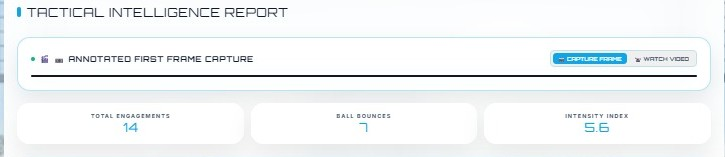
\includegraphics[width=0.90\textwidth]{images_chap3/statistic_A.jpeg}
  \caption{Bloc A — KPIs globaux du match}
  \label{fig:blockA}
\end{figure}

\subsubsection*{Bloc B — Tableau de score}
 
Affichage du score en temps réel entre \textbf{Team Gold} (Opérateurs 3 \& 4) et
\textbf{Team Blue} (Opérateurs 1 \& 2), avec un code couleur distinctif mis à jour
automatiquement par le module de détection de points.

\begin{figure}[H]
  \centering
  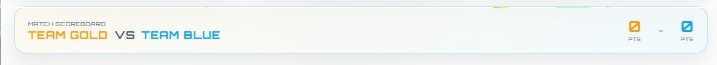
\includegraphics[width=0.90\textwidth]{images_chap3/statistic_B.jpeg}
  \caption{Bloc B — Tableau de score}
  \label{fig:blockB}
\end{figure}

\subsubsection*{Bloc C — Cartes statistiques individuelles (4 joueurs)}
 
Chaque joueur est représenté par une carte statistique affichant neuf métriques biométriques
et tactiques :
 
\begin{table}[H]
  \centering
  \renewcommand{\arraystretch}{1.3}
  \begin{tabularx}{\textwidth}{L{3.2cm} X C{1.5cm}}
    \rowcolor{tablehead}
    \textcolor{white}{\textbf{Métrique}} &
    \textcolor{white}{\textbf{Description}} &
    \textcolor{white}{\textbf{Unité}} \\
    \rowcolor{rowalt}
    Points (PTS)      & Score total accumulé pendant le match & — \\
    Rating (\%)       & Note de performance globale normalisée sur 100 & \% \\
    \rowcolor{rowalt}
    Total Strikes     & Nombre total de frappes détectées & — \\
    Max Velocity      & Vitesse de déplacement maximale atteinte & km/h \\
    \rowcolor{rowalt}
    Distance Covered  & Distance totale parcourue sur l'ensemble du match & m \\
    Avg Tempo         & Vitesse de déplacement moyenne pendant les échanges & km/h \\
    \rowcolor{rowalt}
    Net Presence      & Taux de présence en zone de filet & \% \\
    Calories Burned   & Dépense énergétique estimée par intégration de la distance & kCal \\
    \rowcolor{rowalt}
    Overheads Ratio   & Ratio de frappes en hauteur sur le total des frappes & \% \\
  \end{tabularx}
  \caption{Métriques biométriques et tactiques par joueur}
  \label{tab:metriques_joueur}
\end{table}
 
Le joueur affichant le meilleur rating est mis en valeur visuellement par un badge
\textbf{"TOP"} coloré dans l'angle de sa carte. Dans l'exemple fourni, l'Opérateur 2
(Team Blue) se distingue avec \textbf{31 PTS} et un rating de tête, traduisant une
domination tactique et physique sur le match.
 
\begin{figure}[H]
  \centering
  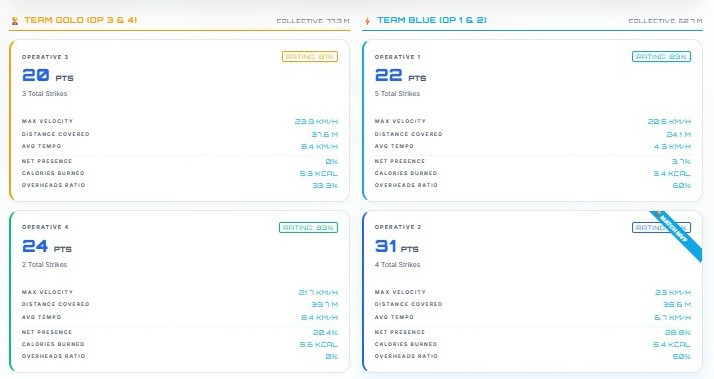
\includegraphics[width=0.90\textwidth]{images_chap3/statistic_C.jpeg}
  \caption{Bloc C — Cartes statistiques individuelles par joueur}
  \label{fig:blockC}
\end{figure}

\subsubsection*{Bloc D — Télémétrie de vitesse}
 
Graphique linéaire multi-courbes généré par Plotly.js, représentant la vitesse de
déplacement (km/h) de chacun des 4 joueurs en fonction du temps (identifiant de frame de
session). Chaque courbe est colorée distinctement selon l'opérateur (OP1, OP2, OP3, OP4).
Ce graphique interactif permet d'identifier :
 
\begin{itemize}[leftmargin=1.5em]
  \item Les pics d'effort correspondant aux sprints défensifs ou aux retours de balle
  \item Les phases de récupération visibles sous forme de plateaux à vitesse nulle ou faible
  \item Les asymétries d'effort entre partenaires d'une même équipe ou entre les deux équipes
\end{itemize}
 
\begin{figure}[H]
  \centering
  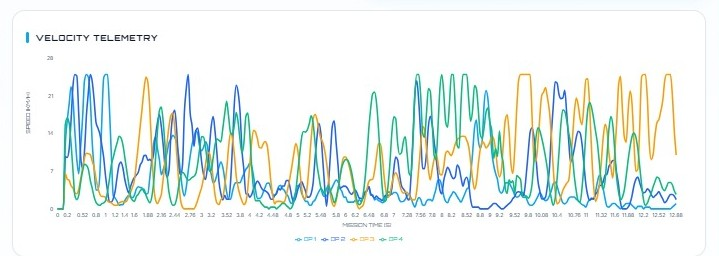
\includegraphics[width=0.90\textwidth]{images_chap3/statistic_D.jpeg}
  \caption{Bloc D — Graphique de télémétrie de vitesse}
  \label{fig:blockD}
\end{figure}

\subsubsection*{Bloc E — Strike Classification}
 
Répartition des types de frappes par joueur, affichée sous forme de badges colorés
comptabilisés pour chaque opérateur : SMASH, FOREHAND, BACKHAND, BANDEJA, LOB. Cette
classification croise la trajectoire de la balle et la posture du joueur au moment de
l'impact pour inférer automatiquement le type de frappe.

\begin{figure}[H]
  \centering
  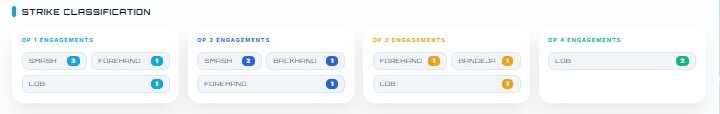
\includegraphics[width=0.90\textwidth]{images_chap3/statistic_E.jpeg}
  \caption{Bloc E — Classification des frappes}
  \label{fig:blockE}
\end{figure}
 
\subsubsection*{Bloc F — Historique des opérations (Recent Operations)}
 
Le bloc \textit{Opérations récentes} affiche les identifiants hexadécimaux des 7 dernières
analyses archivées (ex : \texttt{7C295C}, \texttt{B38164}...). Chaque identifiant correspond
à un fichier JSON stocké dans \texttt{/results\_json/}, permettant de recharger une analyse
passée sans relancer le traitement.
 
% ════════════════════════════════════════════════════════════════════════════
\section{Workflow utilisateur et exemples d'utilisation}
% ════════════════════════════════════════════════════════════════════════════
 
Le workflow complet d'un entraîneur utilisant SmartPlayAI se décompose en cinq étapes
successives :
 
% ─────────────────────────────────────────────────────────────────────────────
% FIGURE 4.5 — Workflow utilisateur
% Remplacez VOTRE_URL_IMAGE_4_5 par l'URL ou le chemin local de l'image
% ─────────────────────────────────────────────────────────────────────────────
\begin{figure}[H]
    \centering
    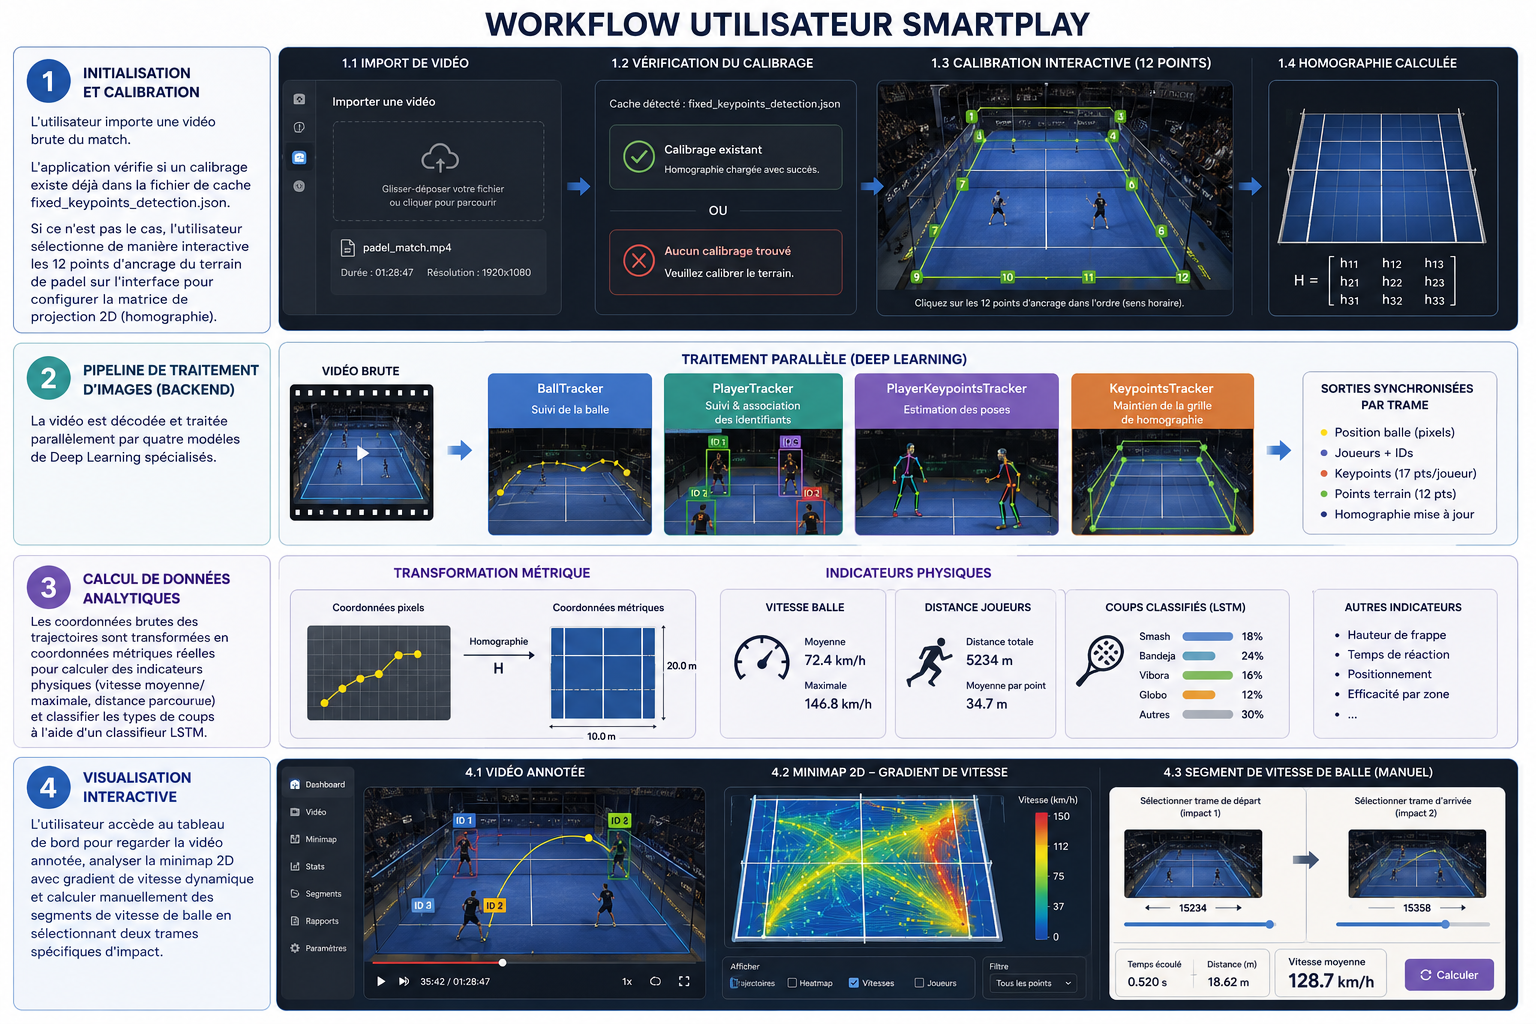
\includegraphics[width=0.90\textwidth]{images_chap3/place_holder.png}
    \caption{Workflow utilisateur complet d'une session d'analyse SmartPlayAI}
    \label{fig:workflow}
\end{figure}

\subsection*{Exemple d'utilisation 1 : analyse post-match d'un tournoi}
 
Un entraîneur reçoit la vidéo \texttt{.mp4} d'un match joué la veille lors d'un tournoi
régional. Il :
 
\begin{itemize}[leftmargin=1.5em]
  \item Importe la vidéo dans le panneau de configuration $\rightarrow$ l'interface confirme
        \textbf{VIDEO SYNCHRONIZED}
  \item Clique sur \textit{Capture Frame} $\rightarrow$ vérifie visuellement que le terrain
        est entièrement couvert
  \item Importe le fichier \texttt{court\_keypoints\_terrain\_A.json} (calibration
        préalablement effectuée pour ce terrain spécifique)
  \item Lance l'analyse via \textbf{LAUNCH NEURAL ANALYSIS} $\rightarrow$ observe le journal
        de mission pendant le traitement ($\sim$3--5 min)
  \item Consulte le rapport final : identifie que l'Opérateur 2 présente un ratio LOB de
        60\% et une vitesse maximale de 23 km/h, révélant une stratégie défensive dominante
\end{itemize}
 
\subsection*{Exemple d'utilisation 2 : suivi longitudinal d'un joueur}
 
L'entraîneur souhaite évaluer la progression d'un joueur sur plusieurs semaines. Il accède
à l'historique via le bloc \textit{Recent Operations} et charge successivement trois analyses
archivées (identifiées par leurs codes hexadécimaux \texttt{7C295C}, \texttt{B38164},
\texttt{C980BD}...) pour comparer l'évolution de la distance couverte, du tempo moyen et du
rating sur trois sessions consécutives.
 
\subsection*{Exemple d'utilisation 3 : calibration d'un nouveau terrain}
 
Pour un terrain n'ayant jamais été analysé, l'entraîneur utilise le champ
\textit{Advanced Parameters (JSON)} pour saisir manuellement les 12 keypoints identifiés
sur la frame capturée :
 
\begin{center}
\begin{lstlisting}[basicstyle=\small\ttfamily, backgroundcolor=\color{black!5},
                   frame=single]
[[145, 892], [1772, 887], [145, 695], [958, 695],
 [1772, 695], [145, 539], [1772, 539], [145, 384],
 [958, 384], [1772, 384], [145, 188], [1772, 183]]
\end{lstlisting}
\end{center}
 
Le système calcule la matrice d'homographie à partir de ces coordonnées et projette le
terrain sur un plan 2D normalisé aux dimensions réglementaires (10m × 20m), permettant
l'expression des métriques de distance et de vitesse en unités physiques réelles.
 
% ════════════════════════════════════════════════════════════════════════════
\section{Évaluation et validation de la solution}
% ════════════════════════════════════════════════════════════════════════════

Cette section a pour objectif d'évaluer la capacité de SmartPlayAI à répondre aux
exigences fonctionnelles et techniques définies au début du projet. L'évaluation
porte à la fois sur la validation des fonctionnalités offertes à l'utilisateur et
sur l'analyse des performances du pipeline d'intelligence artificielle dans
différentes conditions d'utilisation.

% ────────────────────────────────────────────────────────────────────────────
\subsection{Protocole de validation}
% ────────────────────────────────────────────────────────────────────────────

La validation de SmartPlayAI a été réalisée à travers une série de scénarios
représentatifs d'une utilisation réelle de la plateforme. Les tests ont porté sur
l'ensemble de la chaîne de traitement, depuis le chargement des vidéos jusqu'à la
génération des statistiques et des visualisations finales.

Les expérimentations ont été effectuées sur plusieurs vidéos de matchs de padel
enregistrées dans différentes conditions de résolution, d'éclairage et de qualité
d'acquisition. Les métriques observées concernent principalement la robustesse des
modules de détection, la cohérence des événements détectés ainsi que les
performances d'exécution du système.

% ────────────────────────────────────────────────────────────────────────────
\subsection{Validation fonctionnelle}
% ────────────────────────────────────────────────────────────────────────────

Les tests fonctionnels ont permis de vérifier le bon fonctionnement des
principales fonctionnalités développées au sein de SmartPlayAI. Les scénarios
évalués couvrent l'intégralité du \textit{workflow} applicatif : chargement et
lecture des vidéos, sélection des paramètres d'analyse, détection automatique des
joueurs, suivi de la balle, estimation des points clés corporels, génération des
statistiques biomécaniques, visualisation des résultats dans le tableau de bord et
exportation des données d'analyse.

Les résultats obtenus montrent que l'ensemble des fonctionnalités prévues dans le
cahier des charges a été implémenté et intégré avec succès dans une interface
unifiée.

% ────────────────────────────────────────────────────────────────────────────
\subsection{Évaluation des performances}
% ────────────────────────────────────────────────────────────────────────────

L'évaluation des performances a été conduite afin d'estimer les capacités du
système dans différentes configurations matérielles. Un \textit{benchmark} a été
réalisé sur la machine de développement, équipée uniquement d'un processeur
(sans GPU dédié), à l'aide des modèles utilisés en production : YOLO26 pour la
détection des joueurs (\texttt{imgsz=1280}), YOLOv8-Pose pour l'estimation de la
pose (\texttt{imgsz=1280}), un réseau léger pour la détection des points de repère
du terrain (\texttt{imgsz=640}), et TrackNet pour la détection de la balle
(entrée fixe $512 \times 288$).

Les mesures, consignées dans le tableau~\ref{tab:benchmark_cpu}, montrent que la
latence totale sur processeur seul dépasse deux secondes par image, quelle que
soit la résolution d'entrée. Ce résultat s'explique par le fait que les modèles
YOLO et TrackNet effectuent leurs inférences sur des tenseurs de taille fixe,
indépendamment de la résolution source. La résolution n'affecte donc que le coût
de décodage vidéo et de redimensionnement, qui demeure négligeable (moins de
vingt millisecondes même en 4K).

\begin{table}[H]
  \centering
  \renewcommand{\arraystretch}{1.3}
  \begin{tabularx}{\textwidth}{X C{2.2cm} C{2.2cm} C{2.2cm}}
    \rowcolor{tablehead}
    \textcolor{white}{\textbf{Module}} &
    \textcolor{white}{\textbf{720p (ms)}} &
    \textcolor{white}{\textbf{1080p (ms)}} &
    \textcolor{white}{\textbf{4K (ms)}} \\
    \rowcolor{rowalt}
    Décodage \& Redimensionnement & 2,2 & 3,8 & 16,3 \\
    Détection joueurs — YOLO26 (\texttt{imgsz=1280}) & 794,7 & 669,2 & 660,7 \\
    \rowcolor{rowalt}
    Estimation pose — YOLOv8-Pose (\texttt{imgsz=1280}) & 856,6 & 698,0 & 682,6 \\
    Détection terrain — YOLOv8 léger (\texttt{imgsz=640}) & 61,4 & 35,0 & 39,0 \\
    \rowcolor{rowalt}
    Détection balle — TrackNet ($512\times288$, fixe) & 747,1 & 723,5 & 701,6 \\
    \rowcolor{tablehead}
    \textcolor{white}{\textbf{Total pipeline / image}} &
    \textcolor{white}{\textbf{2\,461,9}} &
    \textcolor{white}{\textbf{2\,129,5}} &
    \textcolor{white}{\textbf{2\,100,3}} \\
    \rowcolor{tablehead}
    \textcolor{white}{\textbf{FPS équivalent (CPU)}} &
    \textcolor{white}{\textbf{0,4}} &
    \textcolor{white}{\textbf{0,5}} &
    \textcolor{white}{\textbf{0,5}} \\
  \end{tabularx}
  \caption{Latences mesurées sur CPU par module et par résolution d'entrée}
  \label{tab:benchmark_cpu}
\end{table}

L'utilisation d'un processeur graphique compatible CUDA améliore significativement
les performances et permet d'atteindre environ dix-huit images par seconde pour
des vidéos Full HD, rendant une analyse quasi temps réel envisageable pour un
déploiement opérationnel.

% ────────────────────────────────────────────────────────────────────────────
\subsection{Analyse des résultats}
% ────────────────────────────────────────────────────────────────────────────

L'analyse des expérimentations met en évidence la robustesse globale de
l'architecture proposée. La combinaison des modules de détection, de suivi et
d'analyse permet de produire automatiquement des statistiques cohérentes et
exploitables pour l'analyse des matchs de padel.

Les meilleurs résultats ont été obtenus avec des vidéos Full HD
($1920 \times 1080$ pixels) enregistrées à une cadence comprise entre 30 et
60 images par seconde. Le tableau~\ref{tab:resolution_impact} synthétise l'impact
de la résolution d'entrée sur la qualité de détection et formule les
recommandations opérationnelles correspondantes.

\begin{table}[H]
  \centering
  \renewcommand{\arraystretch}{1.3}
  \begin{tabularx}{\textwidth}{L{3.5cm} C{2.5cm} C{3.5cm} X}
    \rowcolor{tablehead}
    \textcolor{white}{\textbf{Résolution}} &
    \textcolor{white}{\textbf{FPS source}} &
    \textcolor{white}{\textbf{Qualité de détection}} &
    \textcolor{white}{\textbf{Recommandation}} \\
    \rowcolor{rowalt}
    480p ($854\times480$)    & 30    & Insuffisante & Non recommandé \\
    720p ($1280\times720$)   & 30    & Acceptable   & Minimum opérationnel \\
    \rowcolor{rowalt}
    1080p ($1920\times1080$) & 30–60 & Bonne        & Recommandé (\textit{sweet-spot}) \\
    4K ($3840\times2160$)    & 30–60 & Excellente   & Optimal si GPU $\geq$ 8\,Go VRAM \\
  \end{tabularx}
  \caption{Impact de la résolution vidéo d'entrée sur la qualité de détection}
  \label{tab:resolution_impact}
\end{table}

Cette configuration offre un compromis satisfaisant entre précision de détection
et coût de calcul. En deçà de 720p, la balle présente un diamètre apparent
inférieur à trois à cinq pixels, ce qui compromet la fiabilité de la détection
par TrackNet.

% ════════════════════════════════════════════════════════════════════════════
\section{Discussion et limites de la solution}
% ════════════════════════════════════════════════════════════════════════════

% ────────────────────────────────────────────────────────────────────────────
\subsection{Forces et contributions de SmartPlayAI}
% ────────────────────────────────────────────────────────────────────────────

SmartPlayAI présente plusieurs contributions originales par rapport aux solutions
existantes. Premièrement, la plateforme a été conçue spécifiquement pour le
padel, contrairement aux outils généralistes disponibles. Cette spécialisation a
permis d'intégrer des modèles et des traitements adaptés aux caractéristiques
particulières de ce sport, notamment la grande vitesse de déplacement de la balle
et la présence de surfaces vitrées réfléchissantes.

Deuxièmement, l'architecture modulaire facilite l'évolution future du système en
permettant le remplacement ou l'amélioration indépendante de chaque composant
— BallTracker, PlayersTracker, KeypointsTracker et DataAnalytics — sans remettre
en cause l'ensemble du pipeline.

Troisièmement, la plateforme automatise l'intégralité du processus d'analyse,
depuis la vidéo brute jusqu'à la production de statistiques biomécaniques et
d'indicateurs tactiques, sans nécessiter d'intervention manuelle entre les étapes.
Enfin, le recours à des inférences à taille fixe pour les modèles YOLO
(\texttt{imgsz=1280}) et TrackNet ($512\times288$) confère au système un coût de
traitement prévisible et indépendant de la résolution source, ce qui simplifie la
gestion des performances sur différentes configurations matérielles.

% ────────────────────────────────────────────────────────────────────────────
\subsection{Limites techniques identifiées}
% ────────────────────────────────────────────────────────────────────────────

Malgré les résultats obtenus, plusieurs limites subsistent. La détection de la
balle demeure sensible aux situations d'occlusion prolongée, aux réflexions sur
les surfaces vitrées du court ainsi qu'aux conditions d'éclairage défavorables. Si
le filtrage par marges géométriques réduit le nombre de faux positifs, il ne les
élimine pas entièrement lorsque la lumière rasante est particulièrement intense.

Par ailleurs, l'homographie est calculée une seule fois au démarrage du pipeline.
Tout mouvement de caméra au cours d'un enregistrement invalide la projection 2D et
nécessite une nouvelle calibration manuelle, ce qui constitue une contrainte
opérationnelle notable pour un déploiement sur le terrain.

Enfin, les performances du système diminuent lorsque la fréquence d'acquisition
est trop faible. TrackNet est optimisé pour une cadence de 25 à 30 images par
seconde ; en dessous de 15 FPS, les trajectoires deviennent discontinues et
l'interpolation parabolique génère des artefacts visibles sur les statistiques de
vitesse.

% ────────────────────────────────────────────────────────────────────────────
\subsection{Contraintes matérielles et opérationnelles}
% ────────────────────────────────────────────────────────────────────────────

L'exécution complète du pipeline nécessite des ressources matérielles importantes.
Le tableau~\ref{tab:hardware_requirements} présente les exigences minimales et
recommandées pour chaque composant du système, en distinguant le mode CPU seul
(traitement différé) du mode GPU CUDA (traitement quasi temps réel).

\begin{table}[H]
  \centering
  \renewcommand{\arraystretch}{1.3}
  \begin{tabularx}{\textwidth}{L{3.2cm} X X}
    \rowcolor{tablehead}
    \textcolor{white}{\textbf{Ressource}} &
    \textcolor{white}{\textbf{Minimum}} &
    \textcolor{white}{\textbf{Recommandé}} \\
    \rowcolor{rowalt}
    GPU VRAM          & 0 (CPU seul, $<$\,1\,FPS)    & 8\,Go (RTX\,3060, $\sim$18\,FPS) \\
    RAM système       & 16\,Go                        & 32\,Go \\
    \rowcolor{rowalt}
    Résolution vidéo  & 720p ($1280\times720$)        & 1080p ($1920\times1080$) \\
    Fréquence d'images & 25\,FPS                      & 30–60\,FPS \\
    \rowcolor{rowalt}
    Espace disque     & 10\,Go                        & 50\,Go (sorties annotées) \\
    Support CUDA      & Non requis (mode dégradé)     & CUDA\,11.8+ \\
  \end{tabularx}
  \caption{Exigences matérielles minimales et recommandées}
  \label{tab:hardware_requirements}
\end{table}

Sans GPU disposant d'un support CUDA, le pipeline dépasse deux secondes de
traitement par image, rendant toute analyse en quasi temps réel impossible. Pour
un déploiement opérationnel à une cadence supérieure ou égale à quinze images par
seconde, un GPU NVIDIA disposant d'au moins huit gigaoctets de mémoire vidéo est
indispensable. La comparaison détaillée des performances CPU et GPU est présentée
dans le tableau~\ref{tab:cpu_gpu_comparison}.

\begin{table}[H]
  \centering
  \renewcommand{\arraystretch}{1.3}
  \begin{tabularx}{\textwidth}{X C{2.5cm} C{2.8cm} C{2.5cm}}
    \rowcolor{tablehead}
    \textcolor{white}{\textbf{Module}} &
    \textcolor{white}{\textbf{CPU (ms)}} &
    \textcolor{white}{\textbf{GPU estimé (ms)}} &
    \textcolor{white}{\textbf{Accélération}} \\
    \rowcolor{rowalt}
    Détection joueurs — YOLO26        &  795  & $\sim$18 & $\times$44 \\
    Estimation pose — YOLOv8-Pose     &  857  & $\sim$22 & $\times$39 \\
    \rowcolor{rowalt}
    Détection terrain — YOLOv8 léger  &   61  & $\sim$5  & $\times$12 \\
    Détection balle — TrackNet (CNN)  &  747  & $\sim$8  & $\times$93 \\
    \rowcolor{tablehead}
    \textcolor{white}{\textbf{Total pipeline}} &
    \textcolor{white}{\textbf{2\,462}} &
    \textcolor{white}{\textbf{$\sim$55}} &
    \textcolor{white}{\textbf{$\times$45}} \\
    \rowcolor{tablehead}
    \textcolor{white}{\textbf{FPS effectif}} &
    \textcolor{white}{\textbf{0,4\,FPS}} &
    \textcolor{white}{\textbf{$\sim$18\,FPS}} &
    \textcolor{white}{\textbf{—}} \\
  \end{tabularx}
  \caption{Comparaison des temps d'inférence CPU versus GPU par module}
  \label{tab:cpu_gpu_comparison}
\end{table}

La qualité des résultats dépend également de la qualité des vidéos fournies en
entrée. Les conditions d'acquisition recommandées sont détaillées dans les
tableaux~\ref{tab:video_formats} et~\ref{tab:lighting_conditions}, portant
respectivement sur le format de fichier et les conditions de luminosité.

\begin{table}[H]
  \centering
  \renewcommand{\arraystretch}{1.3}
  \begin{tabularx}{\textwidth}{L{2.8cm} L{3cm} X L{3.5cm}}
    \rowcolor{tablehead}
    \textcolor{white}{\textbf{Container}} &
    \textcolor{white}{\textbf{Codec}} &
    \textcolor{white}{\textbf{Avantages}} &
    \textcolor{white}{\textbf{Sources typiques}} \\
    \rowcolor{rowalt}
    MP4 (\texttt{.mp4}) & H.264 (AVC)    & Large compatibilité, décodage rapide, bon ratio qualité/compression & Caméras grand public, smartphones, caméras IP \\
    MOV (\texttt{.mov}) & H.264 / ProRes & ProRes quasi-sans perte, idéal pour capture haute précision         & Caméras professionnelles (Blackmagic, Canon) \\
    \rowcolor{rowalt}
    AVI (\texttt{.avi}) & MJPEG / H.264  & Compression limitée — utile pour tester le pipeline sans artefacts  & Caméras de surveillance ou de laboratoire \\
  \end{tabularx}
  \caption{Formats vidéo supportés et recommandations d'acquisition}
  \label{tab:video_formats}
\end{table}

\begin{table}[H]
  \centering
  \renewcommand{\arraystretch}{1.3}
  \begin{tabularx}{\textwidth}{L{3.5cm} C{2.5cm} X L{4cm}}
    \rowcolor{tablehead}
    \textcolor{white}{\textbf{Situation}} &
    \textcolor{white}{\textbf{Luminosité (lux)}} &
    \textcolor{white}{\textbf{Effet sur le pipeline}} &
    \textcolor{white}{\textbf{Réglage recommandé}} \\
    \rowcolor{rowalt}
    Éclairage naturel doux (indoor)       & 300–500    & Bonne visibilité des lignes, balance de couleur neutre          & ISO 400–800, balance automatique \\
    Lumière forte / plein soleil (outdoor) & $>$\,1\,000 & Reflets et \textit{flare} $\rightarrow$ faux positifs de balle & Filtre polarisant, ISO 200–400, obturateur 1/1\,000\,s \\
    \rowcolor{rowalt}
    Éclairage faible / soirée (indoor)    & $<$\,200   & Bruit vidéo, perte de contraste, balle $<$ 3\,px               & ISO 800–1\,600, LED diffuse ($\sim$500\,lux), gamma $\approx$ 1,2 \\
    Éclairage directionnel / spot         & 500–800    & Ombres nettes perturbant la segmentation du fond                & Diffuseur, filtre médian $3\times3$ avant détection \\
  \end{tabularx}
  \caption{Conditions de luminosité et réglages recommandés pour l'acquisition}
  \label{tab:lighting_conditions}
\end{table}

% ────────────────────────────────────────────────────────────────────────────
\subsection{Perspectives d'amélioration}
% ────────────────────────────────────────────────────────────────────────────

Plusieurs pistes d'amélioration peuvent être envisagées pour renforcer les
capacités et élargir le champ d'application de SmartPlayAI.

Sur le plan de l'optimisation des performances, la conversion des modèles YOLO et
TrackNet au format TensorRT permettrait de réduire la latence GPU d'un facteur
deux à trois supplémentaires. La parallélisation de la détection des joueurs et de
la balle par traitement par lots (\textit{batching}) offrirait une meilleure
utilisation du processeur graphique et faciliterait l'atteinte des trente images
par seconde en continu.

Sur le plan fonctionnel, la suppression de l'étape manuelle de sélection des
points du terrain par une détection automatique des lignes — via un modèle
spécialisé — constituerait une amélioration significative de l'ergonomie de la
plateforme. L'intégration d'un réseau récurrent de type LSTM permettrait en outre
de prédire automatiquement le type de coup effectué (smash, lob, bandeja) à partir
des séquences de points clés corporels.

Sur le plan du déploiement, l'extension du pipeline à des configurations
multi-caméras améliorerait la couverture du terrain et réduirait les zones
d'occlusion. Le portage sur GPU embarqué de type NVIDIA Jetson ouvrirait enfin la
voie à une installation autonome directement sur le court, sans dépendance
vis-à-vis d'un serveur distant. À plus long terme, l'adaptation du système à
d'autres sports de raquette constitue une perspective d'extension naturelle de
l'architecture développée.

% ════════════════════════════════════════════════════════════════════════════
\section{Conclusion}
% ════════════════════════════════════════════════════════════════════════════
 
Ce chapitre a présenté en détail la réalisation de l'interface utilisateur SmartPlayAI, depuis
la définition des spécifications fonctionnelles jusqu'à l'implémentation et la description
des différentes vues de l'application.
 
L'interface se distingue par son approche holistique de l'analyse sportive : elle ne se
limite pas à afficher des statistiques brutes, mais propose un workflow guidé en cinq étapes
permettant à un entraîneur de padel, sans compétences techniques particulières, de piloter
un pipeline d'intelligence artificielle complet et d'en exploiter les résultats de manière
immédiate et lisible.
 
Le panneau de configuration — chargement vidéo, calibration terrain, déclenchement de
l'analyse — et le tableau de bord tactique — KPIs globaux, cartes joueurs, télémétrie
vitesse, classification des frappes — forment un système cohérent et complémentaire, conçu
pour répondre aux besoins réels des entraîneurs lors des phases d'analyse post-match et de
suivi longitudinal des performances.
 
Les choix technologiques retenus (React et Vite en frontend, FastAPI et Python en backend,
YOLO et TrackNet pour l'IA, déploiement via Docker) garantissent à la fois la réactivité de
l'interface, la puissance du traitement et la modularité du système, ouvrant la voie aux
évolutions et aux extensions décrites dans la conclusion générale du rapport.
 
\bigskip
\begin{center}
  \textit{— Fin du chapitre —}
\end{center}
